\section{Задание}

\begin{equation}
    x = \cfrac{t}{t^2 + 1}; \  y = \cfrac{t^2 + 1}{t^3 - t^2 + 2}
\end{equation}

Сначала решим:

\begin{equation}
    x = \cfrac{t}{t^2+1} \implies xt^2 - t + x = 0 \implies t = \cfrac{\pm\sqrt{1 - 4x^2} + 1}{2x}
\end{equation}

Подставим в $y$, здесь фигурные скобки это не и а или:

\begin{equation}
    y = 
    \begin{cases}
        \cfrac{\inner{\cfrac{\sqrt{1 - 4x^2} + 1}{2x}}^2 + 1}{\inner{\cfrac{\sqrt{1 - 4x^2} + 1}{2x}}^3 - \inner{\cfrac{\sqrt{1 - 4x^2} + 1}{2x}}^2 + 2} \\        
        \cfrac{\inner{\cfrac{-\sqrt{1 - 4x^2} + 1}{2x}}^2 + 1}{\inner{\cfrac{-\sqrt{1 - 4x^2} + 1}{2x}}^3 - \inner{\cfrac{-\sqrt{1 - 4x^2} + 1}{2x}}^2 + 2} \\        
    \end{cases}
\end{equation}

\begin{equation}
    y = 
    \begin{cases}
        \cfrac{2 x}{-2 x^2 - (3x - 1) \sqrt{1 - 4 x^2} + x + 1} \\        
        \cfrac{2 x}{-2 x^2 + (3 x - 1) \sqrt{1 - 4 x^2} + x + 1}
    \end{cases}
\end{equation}

\begin{equation}
    0 = 
    \begin{cases}
        y - \cfrac{2 x}{-2 x^2 - (3x - 1) \sqrt{1 - 4 x^2} + x + 1} \\        
        y - \cfrac{2 x}{-2 x^2 + (3 x - 1) \sqrt{1 - 4 x^2} + x + 1}
    \end{cases}
\end{equation}

\begin{figure}[H]
    \centering
    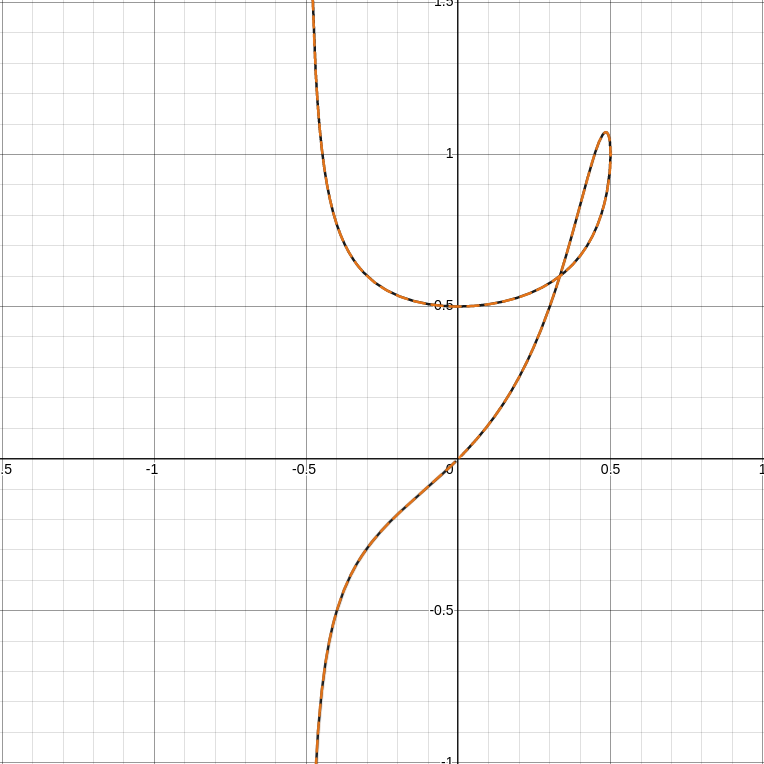
\includegraphics[trim={0 0 0 0},clip,width=\textwidth]{Imgs/Plot.png}
    \label{pict}
    \caption{\href{https://www.desmos.com/calculator/8axpewyf19}{Ссылка на график}}
\end{figure}

